\documentclass[conference]{IEEEtran}
\IEEEoverridecommandlockouts
% The preceding line is only needed to identify funding in the first footnote. If that is unneeded, please comment it out.
\usepackage{cite}
\usepackage{amsmath,amssymb,amsfonts}
\usepackage{graphicx}
\usepackage{textcomp}
\usepackage{xcolor}
\def\BibTeX{{\rm B\kern-.05em{\sc i\kern-.025em b}\kern-.08em
    T\kern-.1667em\lower.7ex\hbox{E}\kern-.125emX}}
\title{
\vspace{1cm}
{\includegraphics[width=0.15\textwidth]{/storage/emulated/0/Screenshot_2024_1018_113636.jpg} \\ Seven Segment Display through Arduino} }
\author{Shaik Mohisena Tabassum \\ Roll No: FWC22279 \\ shaikmohisena123@gmail.com}
 \begin{document}
\maketitle
 \section {ABSTRACT}
 The document shows the connection between the Arduino and Seven segment display.
\section{COMPONENTS}
The seven segment display as shown in Fig.1 has eight pins, $a, b, c, d, e, f, g$ and $dot$ that take an active $LOW$ input, i.e. the LED will glow only if the input is connected to ground. Each of these pins is connected to an LED segment. \\
The Arduino Uno has some ground pins, analog input pins $A0-A3$ and digital pins $D1-D13$ that can be used for both input as well as output. It also has two power pins that can generate $3.3V$ and $5V$.In the following exercises, only the $GND, 5V$ and digital pins will be used. \\
The required components list is given in Table: I. The pin diagram of the seven segment display is shown in Fig.1.
\begin{figure}[h]
\centering
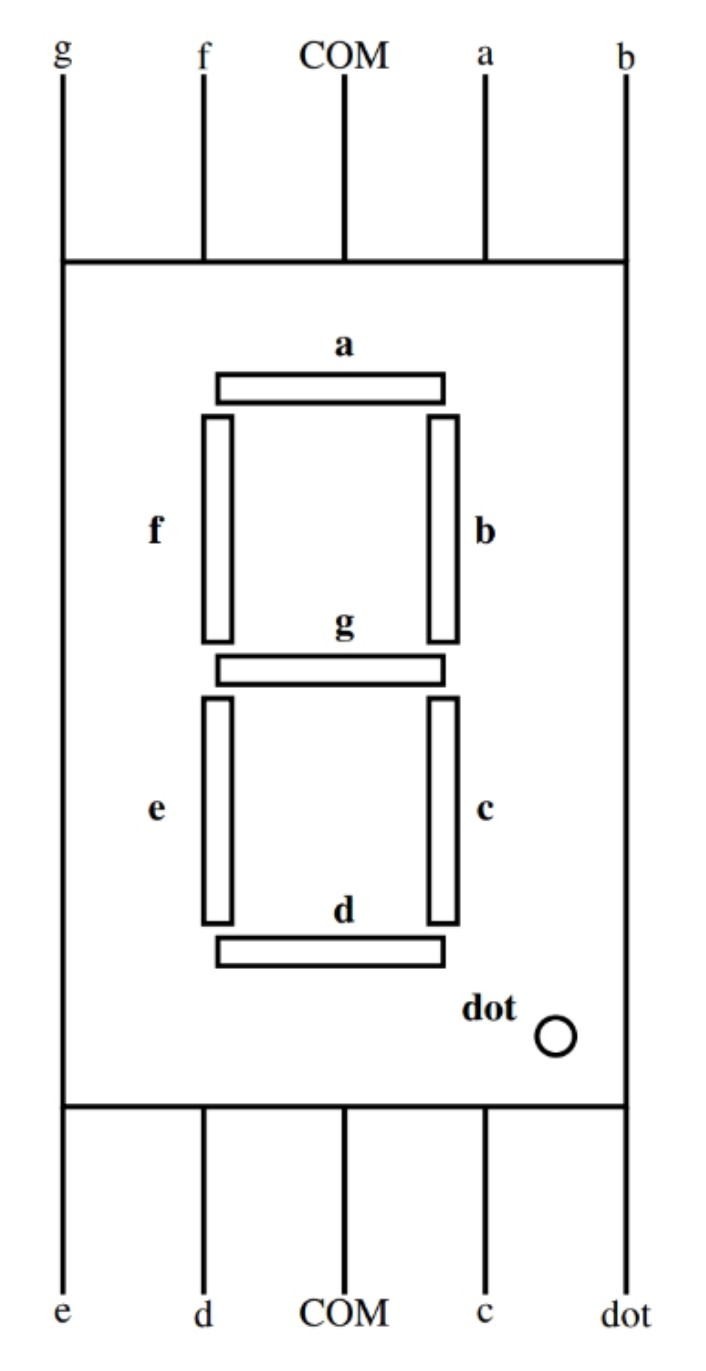
\includegraphics[width=0.30\textwidth]{Screenshot_2024_1021_104340.jpg}
\caption{\label{fig:Gates}}
\end{figure}
 \begin{table} [htbp]
\centering
\begin{tabular}{| c | c | c |} \hline
\textbf{Components} & \textbf{Value} & \textbf{Quantity} \\\hline
Seven Segment Display & & 1 \\ \hline
Arduino & UNO & 1 \\ \hline
Jumper Wires &  & 10 \\ \hline
Breadboard & & 1 \\ 
\hline
\end{tabular}
\vspace{0.1cm}
\caption{\label{tab:widgets}}
\end{table}
\section{PROCEDURE}
Make the connections between Arduino and Seven segment display as per the Table: II.
 \begin{table}[htbp]                                       
\centering                                                          
\begin{tabular}{| c | c |} \hline                                
	\textbf{Arduino Pin} & \textbf{Display}  \\\hline 
D2 & a  \\ \hline                          
D3 &  b \\ \hline                          
D4 & c \\ \hline     
D5 & d \\ \hline
D6 & e \\ \hline
D7 & f \\ \hline
D8 & g \\ \hline
5 V  & COM \\ \hline                         
gnd  & dot \\ \hline                                                               
\end{tabular}                                                        
\vspace{0.1cm}                                                       
\caption{\label{tab:widgets}}                                       
\end{table}
\section{RESULTS}
Download the code given in the link below and execute them to see the output as shown in Fig.2 by observing in seven segment display. 
 \\ https://github.com/Tabassum4930/FWC-1/blob/main/Ide/Seven-seg/Code.cpp
\begin{figure}[h] 
	\centering 
	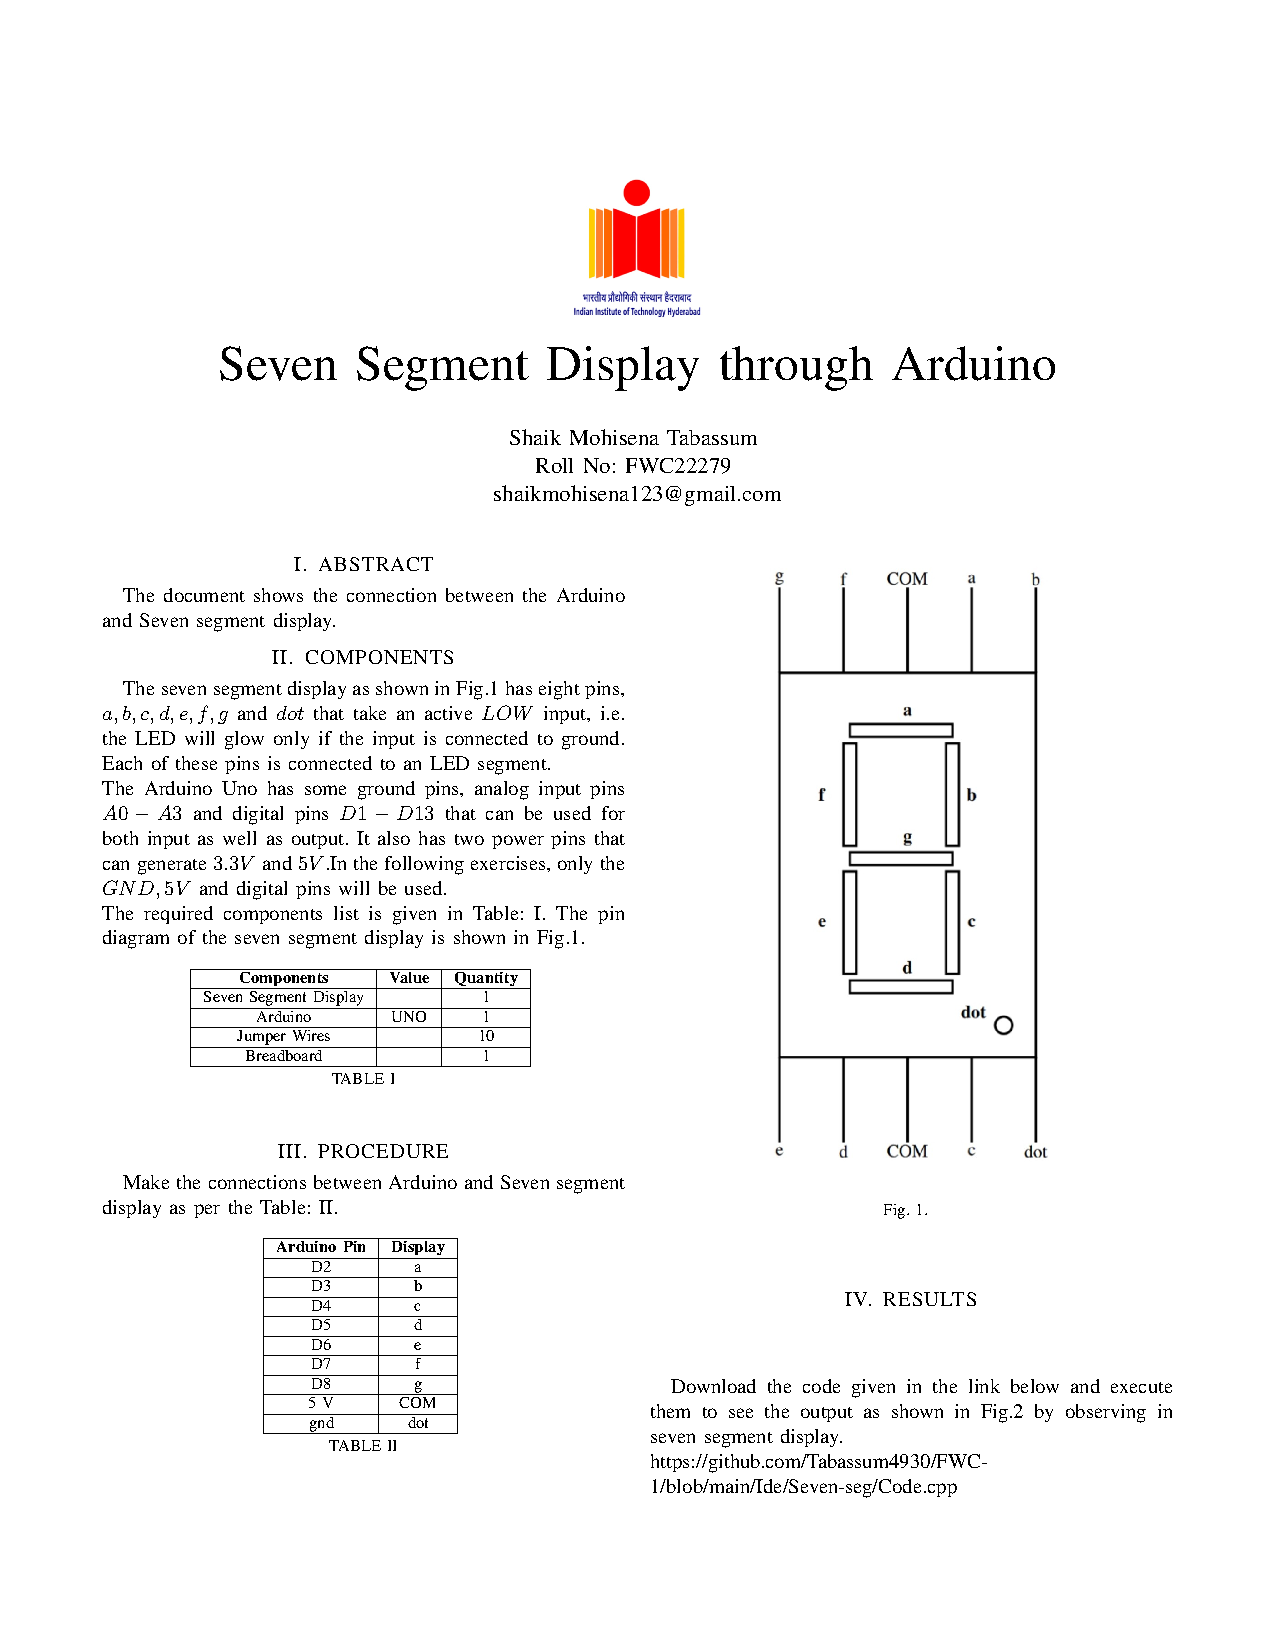
\includegraphics[width=0.35\textwidth]{/storage/emulated/0/internship/seven_seg.jpg}
	\caption{\label{fig:Gates}}    
\end{figure}
\section{CONCLUSION}
The Seven Segment display can be utilized in several applications in order to observe the outputs. Therefore, it is an essential component in the experimentation of digital circuits.
\end{document}
